\documentclass[12pt
,a4paper
,titlepage
,twoside
%,openany % ouvre les sections indifféremment sur la page de gauche ou de droite
]{book}

% Paramétrages de la langue et de l'encodage
\usepackage[utf8]{inputenc}
\usepackage[french]{babel}
\usepackage[T1]{fontenc}

% formules mathématiques
\usepackage{amsmath}
\usepackage{amsfonts}
\usepackage{amssymb}

% gestion des graphiques
\usepackage{graphicx}

% Gestion des couleurs
\usepackage[usenames,dvipsnames]{xcolor}

% Redefinition des liens web
\usepackage{url}
\usepackage[colorlinks=false,urlbordercolor=white,linkbordercolor=white]{hyperref}

% Définition des marges de la page
\usepackage[left=2cm,right=2cm,top=2cm,bottom=2cm]{geometry}

% Polices de caractères
\usepackage{lmodern}
\usepackage{mathptmx} % times, y compris dans les formules mathématiques

% Insertion de code source dans le texte, à utiliser avec \begin{lstlisting} et \lstset{java|html|php...}
\usepackage{listings}

% Définition des entêtes
\usepackage{fancyhdr}
\pagestyle{fancy}

% Redéfinition des titres de section
\usepackage{titlesec}

% Insertion de graphiques à des emplacements définis
\usepackage[abs]{overpic}

% règles typographiques de l'Imprimerie nationale
\usepackage[all]{nowidow}
\usepackage[
% frenchchapters renomme le premier chapitre, mais :
%	- cela pose problème dans la table des matières
%	- cela ne peut être utilisé qu'avec la renumérotation des chapitres activée
%frenchchapters,
parindent,
lastparline,
hyphenation
]{impnattypo}

% Renumérotation des chapitres
%\renewcommand{\thesection}{\Alph{section})}
%\renewcommand{\thesubsection}{\arabic{subsection} -}
%\renewcommand{\thesubsubsection}{\alph{subsubsection} -}
%\usepackage{engrec}
%\renewcommand{\theparagraph}{\engrec{paragraph})}
%\setcounter{secnumdepth}{4}

% Génération du code Ipsum lorem
\usepackage{blindtext}



% Definition des couleurs IRSTEA
\definecolor{titreColor}{RGB}{0,58,128}  % Marine
\definecolor{stitreColor}{RGB}{0,158,224}  % Ocean
\definecolor{auteurColor}{RGB}{0,58,128}     % Marine
\definecolor{texteColor}{RGB}{164,196,0}     % Prairie

% Definition des chapitres
\titleformat{\chapter}[display]
{\normalfont\Large\filcenter\sffamily}
%{\titlerule[1pt]%
% \vspace{1pt}%
% \titlerule
% \vspace{1pc}%
{
 \Large\color{titreColor}{
 %\MakeUppercase{\chaptertitlename}
 \chaptertitlename~\thechapter}
 }
{1pc}
%{\titlerule
%% \vspace{1pc}%
 \Huge

\titleformat{\section}
{\color{titreColor}\normalfont\Large\bfseries\sffamily}
{\color{titreColor}\thesection}{1em}{}

\titleformat{\subsection}
{\color{stitreColor}\bfseries\sffamily}
{\color{stitreColor}\thesubsection}{1em}{}

% Bibliographie
% natbib est indispensable si la biblio contient des accents
% Options pour natbib (extrait de http://merkel.zoneo.net/Latex/natbib.php)
%    round: (par défaut) pour des parenthèses arondies (());
%    square: pour des crochets ([]);
%    curly: pour des accolades ({});
%    angle: pour des équerres (<>) ;
%    colon: (par défaut) pour séparer les citations multiples par deux points (:);
%    comma: pour utiliser une virgule comme séparateur;
%    authoryear: (par défaut) pour des citations auteurs-année;
%    numbers: pour des citations numériques;
%    super: pour des citations numériques en exposant, comme dans Nature;
%    sort: ordonne les citations multiples dans l'ordre dans lequel elles apparaissent dans la bibliographie;
%    sort&compress: comme sort mais en plus les citations numériques multiples sont comprimées, si possible (3-6, 15, par exemple);
%    longnamesfirst: transforme la première citation à une référence en une version étoilée (avec la liste complète des auteurs) et le citations suivantes normales (liste abbrégée);
%    sectionbib: pour redéfinir \thebibliography pour avoir une \section* à la place d'un \chapter*; valide seulement pour les classes de document possédant la commande \chapter; à utiliser avec le paquetage  chapterbib;
%    nonamebreak: garde tous les noms d'auteurs d'une citation sur une même ligne; celà cause des problèmes de débordement, mais permet de résoudre certains problèmes liés à hyperref.

% En cas de souci, supprimez les fichiers .aux et .bbi après modification des paramètres
\usepackage[square,sort,comma,numbers]{natbib}
% styles natbib natifs : abbrvnat, plainnat, unsrtnat
\bibliographystyle{unsrtnat}
\usepackage{hypernat}
% Ajout de la référence à la bibliographie dans la table des matières
\usepackage[nottoc, notlof, notlot]{tocbibind}

%Données de titre et d'auteur pour la page de garde
\newcommand{\titre}{Logiciel COLLEC}
\newcommand{\sousTitre}{Installation et configuration}
\newcommand{\auteur}{Éric Quinton}
\newcommand{\dateModif}{\today}


\begin{document}
%Supprime les veuves et orphelines
\widowpenalty=10000
\clubpenalty=10000
\raggedbottom 

% Integrer la page de garde
%\setcounter{page}{0}
\thispagestyle{empty}
% Logo IRSTEA
\vspace{-2cm}
\hspace{-2cm}

\includegraphics[width=3.06cm,height=3.06cm,keepaspectratio]{logo_irstea}%


\vspace*{4cm}
\hspace{5cm}
\setlength\unitlength{1mm}
% Logo de titre
\begin{overpic}[width=9.44cm,height=9.57cm,keepaspectratio]{logo_fond_droite.png}
% Titre du document
\put(-50,50){
\begin{minipage}{0.7\linewidth}
\Huge\flushright \color{titreColor}{\bfseries\sffamily\titre{}}\\
% sous-titre du document
\color{stitreColor}{\Large \bfseries\sffamily\sousTitre{}}
\end{minipage}
}
\end{overpic}

%  date et auteur
% creation de l'espace a gauche
\vspace*{1cm}
\begin{minipage}{0.5\linewidth}
\hfill
\end{minipage}
% positionnement
\begin{minipage}{0.5\linewidth}\flushleft{
% Date
\textcolor{auteurColor}{\Large\sffamily\dateModif{}}\\
\vspace*{0.1cm}
% Auteur
\textcolor{auteurColor}{\Large\sffamily\auteur{}}\\
\vspace{0.5cm}
% Adresse
\textcolor{texteColor}{\sffamily\textbf{IRSTEA} - Centre de Bordeaux\\
50, avenue de Verdun, Gazinet\\
33612 CESTAS Cedex }
}
\end{minipage}
% Ligne de logos
\begin{minipage}{\linewidth}

% logos complémentaires
%\vspace{3cm}
%\hspace{2cm}
%\includegraphics[width=3cm,height=3cm,keepaspectratio]
%{emplacement_logo}%
%\vspace{-1cm}
%\hspace{1cm}
%\includegraphics[width=3cm,height=3cm,keepaspectratio]
%{emplacement_logo}%
%\vspace{-1cm}
%\hspace{1cm}
%\includegraphics[width=3cm,height=3cm,keepaspectratio]
%{emplacement_logo}%
\end{minipage}
% Définition des entêtes
\fancyhead{}
\fancyhead[CO]{\leftmark\sffamily}
\fancyhead[CE]{ \sffamily\titre{}}
\fancyfoot[CO]{\sffamily\thepage}
\fancyfoot[CE]{\sffamily\thepage}
% Redéfinition de \cleardoublepage pour créer une page totalement vide
\makeatletter
\def\cleardoublepage{\clearpage\if@twoside \ifodd\c@page\else
  \hbox{}
  \vspace*{\fill}

  \vspace{\fill}
  \thispagestyle{empty}
  \newpage
  \if@twocolumn\hbox{}\newpage\fi\fi\fi}
\makeatother

% \cleardoublepage permet de générer une page vide 
% si le chapitre ne commence pas sur la page de droite

% Ajout d'un préambule
\frontmatter
\cleardoublepage

% Table des matières
\tableofcontents


% Début réel du texte
\mainmatter
%\cleardoublepage

\chapter{Besoins nécessitant l'utilisation de services web}

\section{Définitions}

\begin{description}
\item[uid:] identifiant unique numérique au sein d'une base de données d'un échan\-tillon ;
\item[guid:] identifiant de type UUID\footnote{Les codes de type GUID ou UUID sont générés à partir de fonctions aléatoires ou cryptographiques, et garantissent qu'ils sont uniques quelle que soit la base de données qui les ont générés. Ainsi, il n'est pas possible d'obtenir deux codes identiques pour deux échantillons différents, ce qui permet de les identifier de manière sûre, comme pourrait le faire l'ADN pour des êtres humains.}, qui garantit de manière certaine l'identification d'un échantillon ;
\item [identifier :] identifiant \og métier \fg{} d'un échantillon;
\item [données \og métier \fg{} :] données permettant de caractériser un échantillon selon les critères nécessaires à son exploitation : contexte spécifique d'acquisition, taxon, données physico-chimiques ou biologiques, etc.
\item [instance, serveur, base de données, application :] implémentation d'une solution de gestion d'échantillons capable soit de fournir des services web, soit d'interroger des services web pour récupérer des informations.
\end{description}
\section{Présentation}
Collec est un logiciel de gestion de collections d'échantillons, dont l'objectif principal consiste à permettre de retrouver rapidement un échantillon stocké ou de récupérer les informations générales le concernant.

Écrit en PHP, les données sont stockées dans une base de données PostgreSQL. Le code de l'application est disponible à l'adresse \url{https://gitlab.com/Irstea/collec}. Il est disponible sous licence AGPL.

Le logiciel est bâti sur un modèle MVC, tous les accès étant gérés par l'appel à des modules déclarés dans un fichier spécifique. Il ne gère pas initialement les URL conviviales (implémenté à partir de la version 1.1).

La gestion matérielle des échantillons de laboratoire (ou d'expérimentations scientifiques) est une fonctionnalité largement demandée, mais peu couverte jusqu'à présent par les logiciels disponibles, et particulièrement dans le domaine de l'\textit{Open Source}. Collec, dont la première version remonte à l'automne 2016, fait l'objet d'un réel intérêt de la part de la communauté scientifique, ses fonctionnalités et sa facilité d'utilisation le rendant attractif.

Toutefois, il n'est pas conçu comme un système global de gestion de données à la fois techniques -- stockage des échantillons -- et de résultats d'analyse par exemple (pas d'informations métiers complexes\footnote{Dans la pratique, à partir de la version 1.1, il est possible de renseigner quelques informations métiers, mais de manière relativement frustre et sans permettre la complexité des actions envisageables avec des bases de données dédiées.}).
Il n'est pas non plus prévu de mettre en place un hébergement centralisé qui permettrait de gérer tous les échantillons de la sphère de recherche.

\textit{A contrario}, cette organisation permet de créer autant d'instances que néces\-saires, notamment pour gérer des saisies en mode décentralisé (bateau partant en campagne de sondage dans les mers du Sud, collecte d'échantillons depuis des zones non couvertes par Internet, par exemple).

Cette souplesse nécessite de prévoir des mécanismes soit d'interrogation de diverses instances, soit de récupération des informations concernant des échantillons provenant d'autres bases de données. 
Pour harmoniser les échanges ou les interrogations, la technologie des services web s'impose, en raison de la normalisation qu'elle apporte.

\subsection{Technique employée}

Les services web sont basés sur des requêtes HTTP, et échangent les données selon des formats définis. Dans la version actuelle des services web, seul le format Json est implémenté pour l'échange des informations.

\subsection{Forme des URL}
Les URL sont conçues, dans le cadre des services web, sous la forme d'URL conviviales, par exemple : \textit{http://collec/sw/v1/sample/4} pour récupérer l'échan\-tillon numéro 4.

\section{Définition des cas d'utilisation couverts par les services web}

SCHEMA

\subsection{Recherche d'échantillons}
La recherche d'échantillons doit pouvoir s'effectuer selon plusieurs critères :
\begin{itemize}
\item l'identifiant interne (\textit{uid});
\item l'identifiant principal ou des identifiants secondaires;
\item une fourchette de dates de création des échantillons;
\item un type d'échantillons;
\item un projet ou sous-collection;
\item une fourchette d'identifiants internes;
\item un code unique de type GUID ou UUID.
\end{itemize}

Elle retourne une liste d'échantillons correspondant aux critères indiqués. Le détail des informations retournées est spécifié dans la section \ref{sampleSearch}.

Pour permettre cette recherche, d'autres services sont nécessaires, notamment pour récupérer la liste des types d'échantillons ou la liste des projets (ou sous-collections).

\subsection{Liste des projets ou sous-collections}
Ce service doit permettre de récupérer la liste des projets ou sous-collections autorisés pour un utilisateur, pour qu'ils puissent servir dans le cadre de la recherche.

\subsection{Liste des types d'échantillons}
Ce service récupère la liste exhaustive des types d'échantillons utilisés dans l'instance distante, pour une utilisation dans le cadre de la recherche.

\subsection{Liste des types d'identifiants secondaires}
Ce service récupère la liste exhaustive des types d'échantillons secondaires, pour une utilisation dans le cadre de la recherche des échantillons.

\subsection{Récupération des données d'un échantillon}
Ce service permet de récupérer l'ensemble des données concernant un échan\-tillon, y compris les données \og métiers \fg{} si l'utilisateur dispose des droits néces\-saires pour les consulter.

Les données récupérées sont suffisamment complètes pour être intégrées dans l'instance \textit{Collec} courante, par exemple pour éviter de les ressaisir suite au prêt d'un échantillon par un laboratoire.

Elles permettent également une visualisation détaillée de l'échantillon consi\-déré, et contiennent, le cas échéant\footnote{si l'utilisateur dispose des droits adéquats et si l'échantillon dispose de ces informations}, les données \og métiers \fg{} associées.

\subsection{Récupération des données d'une liste d'échantillons}

Il s'agit d'une variante du service web précédent. La liste des échantillons à récupérer est fournie dans une collection Json, soit en utilisant l'UID, soit en utilisant le GUID.

\section{Contraintes liées à la sécurité}

Les instances Collec sont prévues pour donner un accès en lecture à toutes les données des échantillons disponibles, dès lors que l'utilisateur s'est identifié. Cela permet ainsi de connaître, par exemple, le produit utilisé pour la conservation ou d'autres informations nécessaires pour la gestion quotidienne des collections.

Toutefois, les données \og métiers \fg ne sont accessibles qu'aux personnes habilitées à les consulter. Dans la pratique, dans Collec, les échantillons sont associés à un projet, et seuls les utilisateurs rattachés à celui-ci peuvent prendre connaissance de ces informations.
Cela impose une gestion particulière des accès lors de l'interrogation par l'intermédiaire des services web, qui sera décrite dans le chapitre \ref{habilitation}.

Le protocole d'identification des utilisateurs dans l'instance distante est basé sur le protocole Oauth v2.



\chapter{Installer le logiciel}

\section{Consultez la documentation du framework !}

Le logiciel a été conçu à partir du framework \textit{Prototypephp}. La documentation associée \cite{pphp-doc} récapitule l'ensemble des informations nécessaires pour réaliser l'installation générale (configuration du serveur, définition des droits d'accès, etc.).

De nombreuses passages ont été repris ici, mais il n'est pas inutile de se référer au document d'origine. 

\section{Configuration du serveur}
La configuration est donnée pour un serveur Linux fonctionnant avec Ubuntu 16.04 LTS Server. Elle peut bien sûr être adaptée à d'autres distributions Linux. Par contre, rien n'a été prévu pour faire fonctionner l'application directement dans une plate-forme windows, même si, en théorie, cela devrait être possible.

\subsection{Configuration d'Apache}
Les modules suivants doivent être activés :
\begin{lstlisting}
a2enmod ssl
a2enmod headers
a2enmod rewrite
\end{lstlisting}

\subsection{Modules PHP nécessaires}
Modules complémentaires nécessaires :
\begin{itemize}
\item \textit{php-mbstring}
\item \textit{php-pgsql}
\item \textit{php-xdebug} pour les phases de mise au point
\item \textit{php-curl} (ou \textit{php5-curl} pour PHP5) pour l'identification via un serveur CAS.
\end{itemize}
La génération des étiquettes nécessite les paquetages suivants :
\begin{itemize}
\item \textit{php-gd} (ou \textit{php5-gd} pour PHP5)
\item \textit{fop} (qui inclut des bibliothèques java)
\end{itemize}

Le stockage et l'affichage des photos nécessite :
\begin{itemize}
\item \textit{php-imagick} (ou \textit{php5-imagick} pour PHP5)
\end{itemize}

\subsection{Configuration de l'hôte virtuel et de SSL}
L'application ne fonctionne qu'en mode SSL, les cookies de session n'étant pas transmis sur des liens non chiffrés. Voici un exemple de configuration à insérer dans le fichier \textit{/etc/apache2/sites-available/default-ssl}
\begin{lstlisting}
    <Directory /var/www/html>
        Options FollowSymLinks MultiViews
        AllowOverride all
        Order allow,deny
        allow from all
    </Directory>

    SSLProtocol All -SSLv2 -SSLv3
    SSLHonorCipherOrder On
    SSLCipherSuite ECDHE-RSA-AES128-SHA256:AES128-GCM-SHA256:HIGH:
    !MD5:!aNULL:!EDH:!RC4
    SSLCompression off
\end{lstlisting}

La chaîne \textit{SSLCipherSuite} est donnée à titre d'exemple, d'autres configurations plus modernes peuvent être implémentées (\textit{cf.} \cite{tls}).

Pour activer le mode SSL dans Apache :
\begin{lstlisting}
chmod -R g+r /etc/ssl/private
usermod www-data -a -G ssl-cert
a2ensite default-ssl
service apache2 restart
\end{lstlisting}


\subsection{Configuration du dossier d'installation}

\subsubsection{Mécanisme pour faire cohabiter plusieurs instances avec le même code}
\label{dnsmultiple}
Il est possible d'utiliser le même code applicatif pour alimenter des bases de données différentes (ou des données stockées dans des schémas différents). Cette fonctionnalité est basée sur l'attribution d'entrées DNS différentes. 

Le mécanisme est décrit dans le schéma \ref{dnsmultipleschema}, page \pageref{dnsmultipleschema}.

\begin{figure}[H]
\label{dnsmultipleschema}
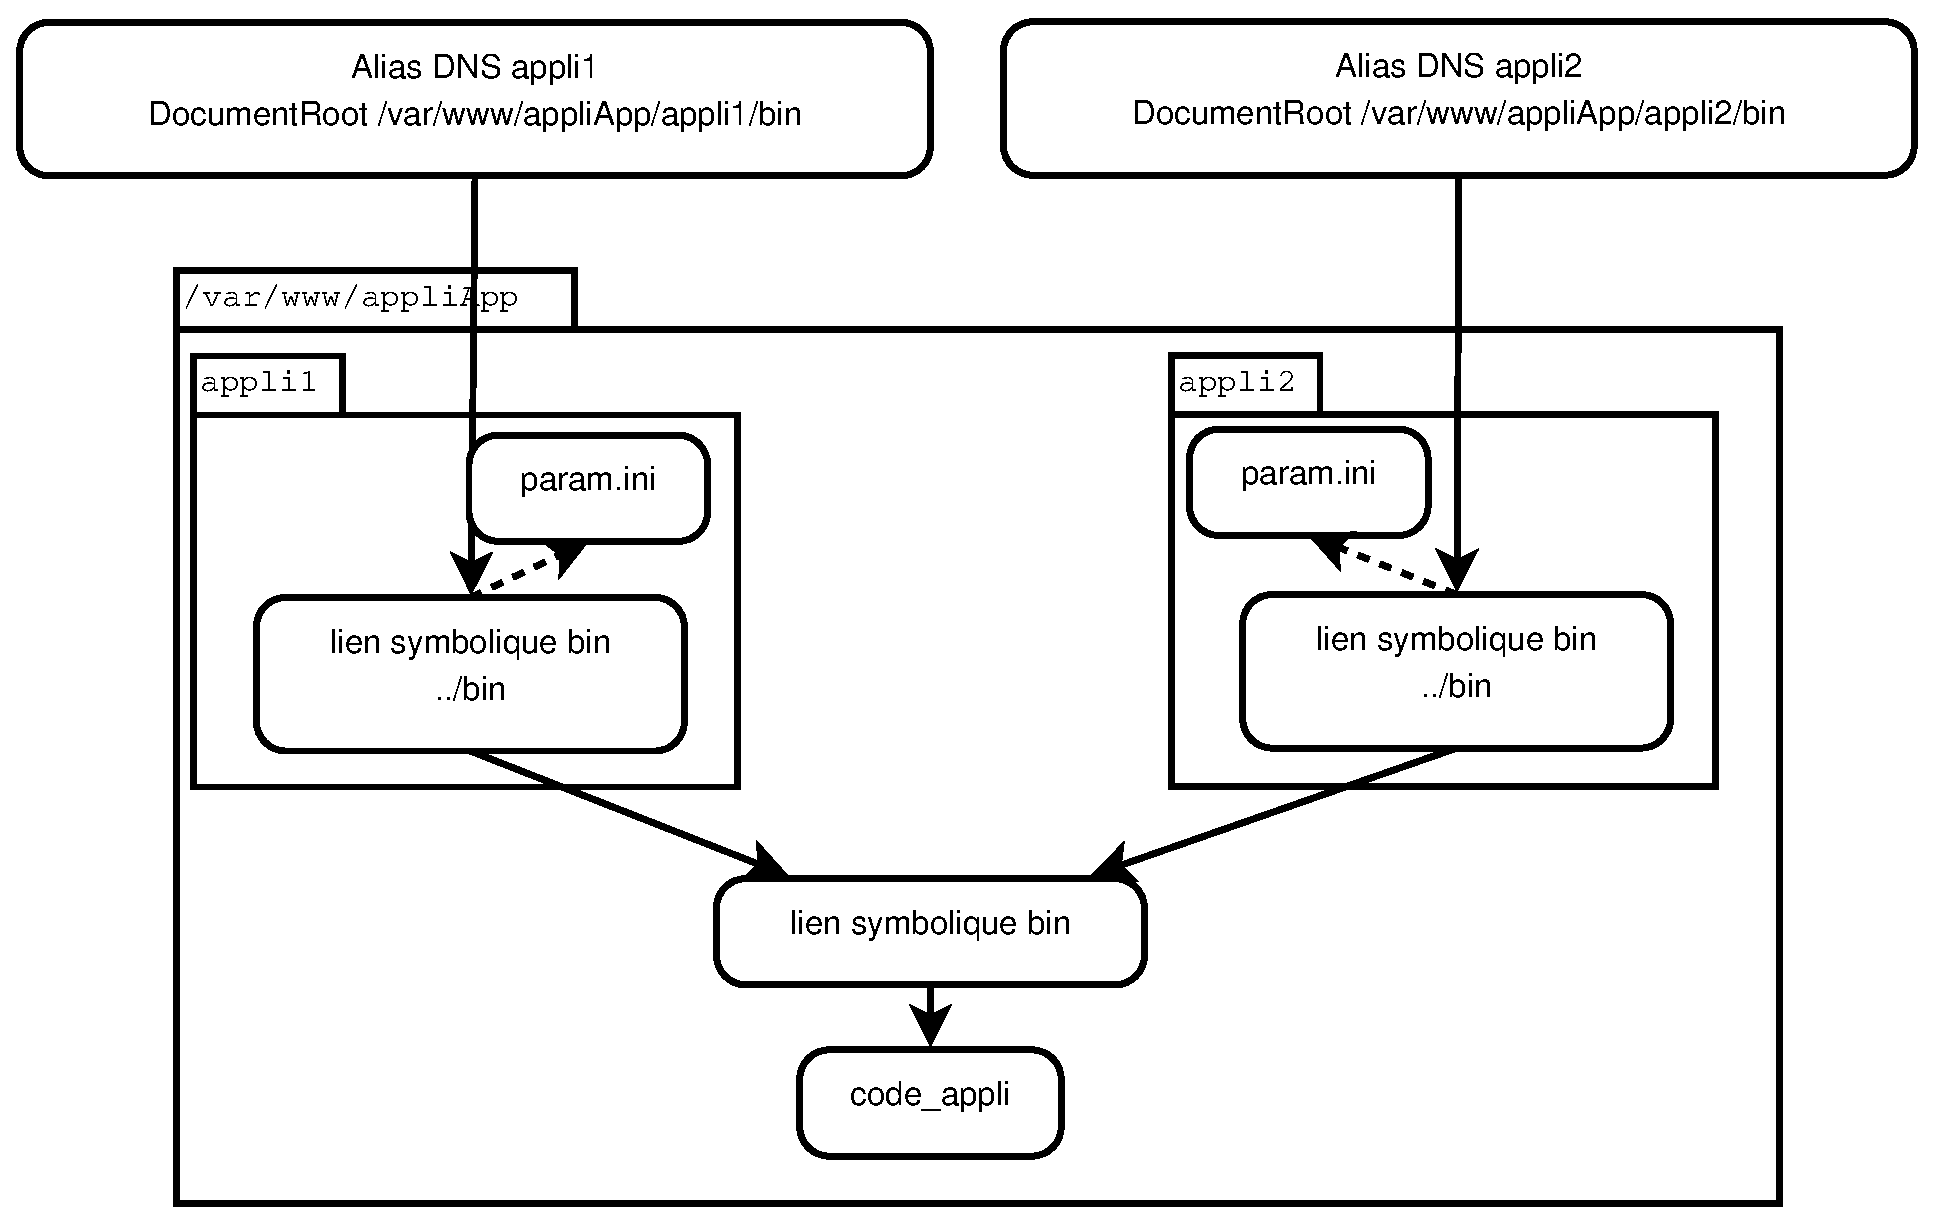
\includegraphics[width=\linewidth]{images/dnsmultiple}
\caption{Schéma général d’implémentation pour utiliser le même code avec des noms d’application et des jeux de données différents}
\end{figure}

Dans le paramétrage de l’alias DNS (en principe, dans \textit{/etc/apache2/sites-available}), l’application pointe vers le dossier \textit{/var/www/appliApp/appli1/bin}. \textit{/var/www} correspond à la racine du site web, \textit{appliApp} au dossier racine de l’application, \textit{appli1} au dossier spécifique de l’alias DNS. Ce dossier \textit{appli1} ne contient que deux fichiers : \textit{param.ini}, qui contient les paramètres spécifiques, et \textit{bin}, qui est un lien symbolique vers le dossier \textit{../bin}.

Le dossier \textit{../bin} (donc, dans\textit{ /var/www/appliApp}) est lui aussi un alias qui pointe vers le code réel de l’application, ici \textit{code\_appli}. Le fichier \textit{param.inc.php} décrit l’entrée suivante : 
\begin{lstlisting}
$paramIniFile = "../param.ini"; 
\end{lstlisting}

Le fichier \textit{param.ini} sera cherché dans le dossier parent du code de l’application, c’est à dire soit dans \textit{appli1}, soit dans \textit{appli2} dans cet exemple. Il suffit qu’il contienne les paramètres adéquats pour rendre l’application utilisable dans des contextes différents à partir du même code initial.



Le fichier \textit{param.ini} est le dernier qui est traité par l'application pour récupérer les paramètres. Ceux-ci sont lus dans l'ordre suivant :

\textbf{param/param.default.inc.php $\rightarrow$ param/param.inc.php $\rightarrow$ ../param.ini}

\textit{param.ini} contiendra les entrées spécifiques liées au DNS utilisé pour accéder à l'application, en principe tout ou partie de celles-ci :
\begin{lstlisting}
APPLI_titre=Gestion des collections EABX
BDD_schema=col, public, gacl
BDD_login=compte_de_connexion
BDD_passwd=mot_de_passe_de_connexion
BDD_dsn=pgsql:host=serveur;dbname=base_de_donnees;sslmode=require
GACL_aco=col
APPLI_code=proto
\end{lstlisting}



\subsubsection{Droits à attribuer au serveur web}

Le serveur web doit pouvoir accéder en lecture à l'ensemble des fichiers de l'application, et en écriture à deux dossiers :
\begin{itemize}
\item \textit{display/templates\_c} : fichier utilisé par Smarty pour compiler les modèles de documents HTML ;
\item \textit{temp} : dossier de génération des images et des fichiers temporaires.
\end{itemize}

Voici un exemple de script utilisé pour positionner les droits :

\begin{lstlisting}
#!/bin/bash
cp ../param/* param/
chmod -R 770 .
setfacl -R -m u:www-data:rx .
setfacl -R -m d:u:www-data:rx .
mkdir display/templates_c
setfacl -R -m u:www-data:rwx display/templates_c
setfacl -R -m d:u:www-data:rwx display/templates_c
setfacl -R -m u:www-data:rwx temp
setfacl -R -m d:u:www-data:rwx temp
setfacl -R -m d:o::- .
rm -Rf database
rm -Rf test
rm -f param.ini
\end{lstlisting}

Dans cet exemple, le dossier \textit{../param} contient le fichier \textit{param.inc.php}, qui dispose des paramètres spécifiques à l'implémentation.

Le script est à lancer à la racine du dossier contenant l'application.

\section{Configurer l'application}

L'application est configurable par l'intermédiaire de trois fichiers, comme nous venons de le voir :

\textbf{param/param.default.inc.php $\rightarrow$ param/param.inc.php $\rightarrow$ ../param.ini}

Le premier fichier contient les paramètres par défaut. Il est systématiquement fourni à chaque nouvelle version de l'application.

Le second est spécifique de l'implémentation. Il comprend notamment les informations liées à la connexion à la base de données, à la méthode d'identification, ou à la recherche des attributs dans l'annuaire LDAP. 

le troisième est destiné à offrir la possibilité d'accéder, à partir du même code applicatif, à plusieurs bases de données différentes (\textit{cf.} \ref{dnsmultiple} \textit{\nameref{dnsmultiple}}).

Voici les principaux paramètres utilisés :

\subsection{Connexion à la base de données}

Dans la pratique, deux connexions sont nécessaires : l'une pour accéder à la base des droits, l'autre aux données proprement dites. Voici les paramètres à définir :

\begin{longtable}{|p{5cm}|p{10cm}|}
\hline
\textbf{Variable} & \textbf{Signification} \\
\hline
\endhead
BDD\_login & compte de connexion à la base de données \\
\hline
BDD\_passwd & mot de passe associé\\
\hline
BDD\_dsn & adresse de la base de données sous forme normalisée\\
\hline
BDD\_schema & schéma utilisé (plusieurs schémas peuvent être décrits, en les séparant par une virgule - fonctionnement propre à Postgresql)\\
\hline
GACL\_dblogin & compte de connexion à la base de données des droits\\
\hline
GACL\_dbpasswd & mot de passe associé\\
\hline
GACL\_dsn & adresse normalisée \\
\hline
GACL\_schema & schéma utilisé\\
\hline
GACL\_aco & nom du code de l'application utilisé dans la gestion des droits\\
\hline
\caption{Variables utilisées pour paramétrer les connexions}
\end{longtable}

\subsection{Identification des utilisateurs}

\begin{longtable}{|p{5cm}|p{10cm}|}
\hline
\textbf{Variable} & \textbf{Signification} \\
\hline
\endhead
ident\_type & Type d'identification supporté. L'application peut gérer \textbf{BDD} (uniquement en base de données),\textbf{LDAP} (uniquement à partir d'un annuaire LDAP) \textbf{LDAP-BDD} (d'abord identification en annuaire LDAP, puis en base de données), et \textbf{CAS} (serveur d'identification \textit{Common Access Service}\footnote{serveur externe gérant l'identification des utilisateurs, et renvoyant à l'application le login utilisé})\\
\hline
CAS\_plugin & Nom du plugin utilisé pour une connexion CAS \\
\hline
CAS\_address & Adresse du serveur CAS\\
\hline
CAS\_port & Systématiquement 443 (connexion chiffrée)\\
\hline
LDAP & tableau contenant tous les paramètres nécessaires pour une identification LDAP \\
\hline
privateKey & clé privée utilisée pour générer les jetons d'identification \\
\hline
pubKey & clé publique utilisée pour générer les jetons d'identification \\
\hline
tokenIdentityValidity & durée de validité, en secondes, des jetons d'identification\\
\hline
\caption{Variables utilisées pour paramétrer l'identification}
\end{longtable}

L'application permet de conserver l'identification plus longtemps que celle définie dans le serveur, en rejouant la connexion avec un jeton d'identification chiffré. Cela évite, par exemple, de devoir se ré-identifier toutes les heures si on accède au logiciel à partir d'un terminal mobile (smartphone ou tablette, par exemple).

Les trois dernières variables permettent de configurer ce mode d'identification. Pour plus d'informations, consultez \cite{token}.

\subsection{Configuration de l'accès à l'annuaire LDAP}

Les paramètres LDAP sont stockés dans un tableau :
\begin{lstlisting}
$LDAP = array(
		"address"=>"localhost",
		"port" => 389,
		"rdn" => "cn=manager,dc=example,dc=com",
		"basedn" => "ou=people,ou=example,o=societe,c=fr",
		"user_attrib" => "uid",
		"v3" => true,
		"tls" => false,
		"groupSupport"=>true,
		"groupAttrib"=>"supannentiteaffectation",
		"commonNameAttrib"=>"displayname",
		"mailAttrib"=>"mail",
		'attributgroupname' => "cn",
		'attributloginname' => "memberuid",
		'basedngroup' => 'ou=example,o=societe,c=fr'
);
\end{lstlisting}


L'application peut non seulement identifier les utilisateurs auprès de l'annuaire LDAP, mais également récupérer les groupes auxquels ils appartiennent dans celui-ci.

Voici les paramètres à indiquer dans ce cas de figure : 
\begin{longtable}{|p{5cm}|p{10cm}|}
\hline
\textbf{Variable} & \textbf{Signification} \\
\hline
\endhead
address &  adresse de l'annuaire\\
\hline
port & 389 en mode non chiffré, 636 en mode chiffré\\
\hline
rdn & compte de connexion, si nécessaire \\
\hline
basedn & base de recherche des utilisateurs\\
\hline
user\_attrib & nom du champ contenant le login à tester\\
\hline
v3 & toujours à \textit{true}\\
\hline
tls & \textit{true} en mode chiffré\\
\hline
groupSupport & \textbf{true} si l'application recherche les groupes d'appartenance du login dans l'annuaire\\
\hline
groupAttrib & Nom de l'attribut contenant la liste des groupes d'appartenance\\
\hline
commonNameAttrib & Nom de l'attribut contenant le nom de l'utilisateur\\
\hline
mailAttrib & Nom de l'attribut contenant l'adresse mail de l'utilisateur\\
\hline
attributgroupname & Attribut contenant le nom du groupe lors de la recherche des groupes (cn par défaut)\\
\hline
attributloginname & attribut contenant les membres d'un groupe\\
\hline
basedngroup & base de recherche des groupes \\
\hline
\caption{Variables utilisées pour paramétrer l'accès à l'annuaire LDAP}
\end{longtable}

\subsection{Paramètres spécifiques}
\label{paramspec}

\begin{longtable}{|p{5cm}|p{10cm}|}
\hline
\textbf{Variable} & \textbf{Signification} \\
\hline
\endhead
GACL\_aco & nom du code de l'application utilisé dans la gestion des droits (\textit{cf.} \ref{droits} \textit{\nameref{droits}}, page \pageref{droits} )\\
\hline
APPLI\_code & Code interne de l'application. \textbf{Ce code est essentiel} : il sera inscrit dans les codes-barres générés, pour s'assurer qu'un échantillon est bien issu de la base de données concernée\\
\hline
\caption{Variables spécifiques}
\end{longtable}

\section{Créer la base de données}

La base de données est composée de deux schémas : l'un pour stocker les informations d'identification, les droits d'accès et les traces, l'autre pour les données proprement dites.

Le schéma \textit{public} ne devrait jamais être utilisé pour stocker l'information : réservez-le pour les composants communs, comme Postgis si c'est nécessaire.

Les tables de gestion des droits peuvent être communes à plusieurs jeux / applications différentes : la variable \textit{GACL\_aco} permet de séparer la gestion des droits pour chaque application, tout en travaillant à partir des mêmes utilisateurs (répartis le cas échéant dans des groupes différents selon le jeu de données considéré).

Les scripts de création des schémas dans la base de données sont stockés dans le dossier \textit{install}. 



\subsection{Créer les tables de gestion des droits}
Script à utiliser : \textit{gacl\_create.sql}. Les tables nécessaires vont être créées dans le schéma \textit{gacl} (ne modifiez pas le nom du schéma).

Le script crée un compte d'administration par défaut :
\begin{itemize}
\item login : \textbf{admin}
\item mot de passe : \textbf{password}
\end{itemize}

Il devra être supprimé quand un autre compte d'administration aura été créé.

Lles droits par défaut sont positionnés pour le projet \textit{appli} (variable \textit{\$GACL\_aco} dans les fichiers de paramètres de l'application).


\subsection{Créer les tables applicatives}
Script à utiliser : \textit{col\_create.sql}.

Par défaut, le script crée un schéma appelé \textit{col}. Il est possible de créer plusieurs schémas différents, si l'application supporte plusieurs jeux de données (\textit{cf.} \ref{dnsmultiple} \textit{\nameref{dnsmultiple}}, page \pageref{dnsmultiple}). Dans ce cas de figure, remplacez \textit{col} par le nom du schéma voulu dans les deux premières lignes du script.

\subsection{Login de connexion}

Il est fortement conseillé de créer deux logins de connexion, un pour le schéma des droits, l'autre pour les schémas applicatifs. Ces logins ne doivent pouvoir être utilisés que depuis le serveur web hébergeant l'application.

Cette opération est possible en modifiant le fichier \textit{/etc/postgresql/9.5/main/pg\_hba.conf} selon ce principe :

\begin{lstlisting}
# Connexions pour les serveurs web 
host nom_database userGacl adresse_serveur/32 md5 
host nom_database userData adresse_serveur/32 md5
\end{lstlisting}

et en rechargeant ensuite la configuration de Postgresql avec la commande :
\begin{lstlisting}
service postgresql reload
\end{lstlisting}

\subsection{Droits sur les tables}

Le compte utilisé pour la connexion au schéma des droits doit pouvoir modifier les informations présentes dans l'ensemble des tables de \textit{gacl}. Il ne doit pas pouvoir accéder aux autres schémas (hormis \textit{public}).

Le compte utilisé pour accéder aux schémas des données doit pouvoir modifier l'ensemble des informations dans les schémas de données, et lire la table \textit{gacl.aclgroup}.

Le plus simple est d'utiliser le logiciel \textit{pgAdmin} \cite{pgadmin} pour attribuer les droits.

\subsection{Scripts de modification}

Lors de la livraison de nouvelles versions, il est possible que des scripts de modification soient livrés pour mettre à niveau la base de données. Ces scripts doivent être exécutés dans tous les schémas contenant des données applicatives.

\section{Mise en production}

Une fois l'application configurée, et après avoir créé un nouveau compte d'administration :
\begin{itemize}
\item supprimez le compte \textit{admin}, livré par défaut, qui ne doit pas être conservé. Sa désactivation n'est pas suffisante : si pour une raison ou pour une autre le compte est réactivé, n'importe qui pourra récupérer les droits totaux ;
\item supprimez le dossier \textit{install} qui contient les scripts de création des tables ;
\item déplacez le dossier \textit{database}, qui contient la documentation d'installation et de configuration (elle n'a pas à rester accessible depuis le site web) ;
\item faites une revue des droits, pour vous assurer que tout est correctement configuré.
\end{itemize}

Vous pouvez également tester si la configuration du serveur est correcte en recourant à ZAProxy \cite{zaproxy}, qui analysera la communication entre le serveur et un navigateur et identifiera les problèmes éventuels de non conformité (mauvaise réécriture des entêtes HTML suite à une mauvaise configuration du serveur Apache, par exemple).

\section{Première section}
Référence bibliographique au livre \citet{livre}, à l'article \citet{article}, à la thèse \citep{these}.

La bibliographie utilise le fichier \textit{irstea.bib} dans cet exemple.



% Second chapitre
%\cleardoublepage
\chapter{Second chapitre}
% \input{chapitre2}

%Annexes
\appendix
\chapter{Première annexe}

%Bibliographie
\backmatter
% Integration de la biblio
% Pour insérer toutes les références : 
%\nocite{*}
% Pour intégrer une référence non citée : 
%\nocite{ref}
\nocite{*}
\bibliography{collec}

\end{document}